
\chapter{Make Objects}
The files to be tracked have simply to be mentioned in \TT{add$\_$executable()} CMake takes care of the dependencies. Only the source files \TT{.cpp} have to mentioned, since CMake track the \TT{.hpp} files automatically since they are included in the source-files.
\begin{center}
\tikzset{
	A/.pic={
        code={
\draw[black](0,0)node[rotate=00]{\tiny \texttt{A}};
\draw[black,thick](-0.5,-0.15)rectangle(0.5,0.15);   
							}
	}
}

\tikzset{
	B/.pic={
        code={
\draw[black](0,0)node[rotate=00]{\tiny \texttt{B}};
\draw[black,thick](-0.5,-0.15)rectangle(0.5,0.15);   
							}
	}
}

\tikzset{
	C/.pic={
        code={
\draw[black](0,0)node[rotate=00]{\tiny \texttt{C}};
\draw[black,thick](-0.5,-0.15)rectangle(0.5,0.15);   
							}
	}
}

\tikzset{
	D/.pic={
        code={
\draw[black](0,0)node[rotate=00]{\tiny \texttt{D}};
\draw[black,thick](-0.5,-0.15)rectangle(0.5,0.15);   
							}
	}
}

\tikzset{
	main/.pic={
        code={
\draw[black](0,0)node[rotate=00]{\tiny \texttt{main}};
\draw[black,thick](-0.5,-0.15)rectangle(0.5,0.15);   
							}
	}
}

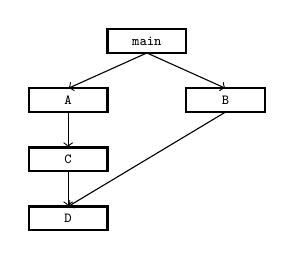
\begin{tikzpicture}
%Gitter
%\draw[step=0.5cm,very thin,black!20] (-6,-6) grid(6,6);
%\draw(-6,0)--(6,0);
%\draw(0,6)--(0,-6);
\path (0,2.75) pic {main};
\path (-1,2) pic {A};
\path (1,2) pic {B};
\path (-1,1.25) pic {C};
\path (-1,0.5) pic {D};
\draw [black,->] (0,2.6)--(-1,2.15);
\draw [black,->] (0,2.6)--(1,2.15);
\draw [black,->] (-1,1.85)--(-1,1.4);
\draw [black,->] (-1,1.1)--(-1,0.65);
\draw [black,->] (1,1.85)--(-1,0.65);
\end{tikzpicture}

\captionof{figure}[D]{Dependency Structure}
\end{center}
\TwinLs
{\TLi{Excerpt Makefile}{./Code/Makefile4.mk}}
{\TLi{Excerpt CMakeList}{./Code/CMakeLists0.txt}}



\newpage
\section{Makefile}
The make-file must be saved as \TT{Makefile} \footnote{it can be saved with arbitrary in this case it has to be called with:\\ \TT{make -f makefileName}}. It is similar to a bash file. The make-file automatically monitors whether a file got changed and therefore needs new compiling or new linking respectively.
\TLi{General form of a make file}{./Code/MakeFile0}
Only if the files listed in dependencies feature a change the action statements will be executed.\\
Variables can be declared they are accessed with \TT{\$(.)}.\\
The following wild cards are used:\\
$ \begin{array}{ll}
\TT{\$} \ \mathtt{\hat{ }} & \text{all Dependencies} \\
\TT{\$<} & \text{first Dependency} \\ 
\TT{\$@} & \text{name of the target}  
\end{array} 
$\\
The dependency structure expressed by suffixes. All \TT{.s} files depend on the \TT{.c} files.
\TLi{}{./Code/SuffixMake.txt}
\TLi{Example}{./Code/daMake.mk}

By default Makefile targets are file-targets. However sometimes Makefile should run commands, that do not represent physical files in the file-system. These special targets need to be declared, so that make does not look for a file. Targets that are not files are called \TT{PHONY}.
%\TLi{Makefile}{./Code/Makefile3}
\newpage

\section{CMake}\label{sec:CMake}
CMake is a program that creates make files according to the CMakeList.txt specifications.\\
Hence the CMake configurations have to be made in the file \TT{CMakelists.txt}.
\begin{center}
\input{./Bilder/Structure7.tex}
%\captionof{figure}[D]{Typical CMake Project-Structure}
\end{center}
\ \\
The $\dagger$ directories are created by the makefile as configured in listing (\ref{Main CMakeList.txt}). CMakeList-files can be sprinkled everywhere desired, we preferably going downwards

\TLi{Main CMakeList.txt}{./Code/CMakeListsMain.txt}
Some Build-types:\\
$\begin{array}{lll}
\TT{Debug} &\TT{=} & \TT{g++ -g}\\ 
\TT{Release} &\TT{=} & \TT{g++ -O3 -DNDEBUG}\\
\TT{None} &\TT{=} & \TT{g++}\\
\end{array}$



\newpage
\TLi{Src  CMakeList.txt}{./Code/CMakeListsSrc.txt}
\TLi{Test CMakeList.txt}{./Code/CMakeListsTest.txt}

%\TLi{Cross Platform Generic CMakeLists.txt}{./Code/CMakeLists11.txt}
%\TLi{Additional CMakeLists.txt in Lib-dir }{./Code/CMakeLists9.txt}

The files to be tracked simply have to be mentioned in \TT{add$\_$executable()} CMake takes care of the dependencies. Only the source files \TT{.cpp} have to mentioned, since CMake track the \TT{.hpp} files automatically since they are included in the source-files.
%\BF{CMakeLists.txt}
%\TLi{Generic CMakeLists.txt}{./Code/CMakeLists2.txt}
\TT{include$\_$directories} adds the directory to the list of directories the pre-compiler searches for files.


The CMakeVariable \TT{CMAKE$\_$SOURCE$\_$DIR} contains the address of the directory where the file \TT{CMakeLists.txt} is found. % (\TT{\$...} $/$\TT{Src}).
%\newpage
\TLi{Create a Make File with Cmake}{./Code/CMakeListsExample1.txt}
The parameter given to \TT{cmake} refers to the folder containing \TT{CMakeLists.txt}. Since it is located in one higher hierarchy it holds ..$/$\TT{Src}.
The makefile and some cmake files get created in the Built-directory.
The generator\footnote{Generator meaning make and g++} creating the acutal objects and executable can be chosen explictially on calling cmake. 
\TLi{Create a Make File with Cmake}{./Code/CMakeListsExample2.txt}

\newpage
\subsection{Testing with CMake}
CMake allows to create a test-executables. A passed test is assumed to return \TT{0}. Each test is an entire executable, meaning each test is created in a separate \TT{main}-function. Tester-Examples:\\
\TwinLs
{\CppLi{GenomeTest1.cpp Example}{./Code/GenomeTest1.cpp}}
{\CppLi{GenomeTest2.cpp Example}{./Code/GenomeTest2.cpp}}
The test are started by \TT{make all test}.




\subsection{Plattform specific Commands}
The \TT{CMakeLists.txt} can contain platform specific commands. 
%\TLi{UNIX}{./Code/CMakeLists3.txt}
In order to keep the \TT{CMakeLists.txt} plattform independent the platform can be discoverd, and the respecitve commands can be issued correctly.
\TLi{Detect the OS Compiler}{./Code/CMakeLists5.txt}
\TLi{Plattform specific}{./Code/CMakeLists6.txt}
\newpage







%#http://cpprocks.com/using-cmake-to-build-a-cross-platform-project-with-a-boost-dependency/
%\subsection{CMakeLists.txt}
%\TLi{Generic CMakeLists.txt}{./Code/CMakeListsGeneric.txt}
%\newpage
%\subsubsection{Example:}
%\TLi{CMakeLists.txt}{./Code/CMakeLists.txt}
%\TLi{Create a Make File with Cmake}{./Code/CMakeListsExample.txt}
%$CDT4$ supports CDT 4.0 or higher.
%The last parameter refers to the source files, since they are in the $src$ folder located in one higher hierarchy it holds ..$/$src. \\
%For the Makefile that was generated see (\ref{sec:Makefile}).

